\documentclass[11pt]{book}
%Gummi|063|=)
\title{\textbf{Complete this book }}
\author{Deebul Nair}
\date{}

\usepackage{amsmath}
\usepackage{todonotes}

\usepackage{tikz}
\usepackage{amsmath}
\usetikzlibrary{bayesnet}
\usepackage{tabularx}

\begin{document}

\chapter{In-House Human Presence Model}

Domestic robots in future should be able to gather knowledge about the favourite places of the humans in the home and also the time period when they mostly occupy their favourite places. This acquired knowledge of the human presence patterns shall enable the robots to make better decisions. For example what time particular rooms are unoccupied for cleaning or when to turn on the heater of the room. 

In this chapter we focus on such knowledge accession from observations made by the robot. However, the advancement in long term autonomous navigation \todo{cite} and the rapid adoption of databases in the robots \todo{cite} has not only made it feasible for domestic robots to acquire such knowledge, but also a number of challenges.  In more details, these challenges are the (i) modelling human presence (ii) prediction of future location (iii) learning all these with sparse observations made by the robots. 

Significant progress has been made on a related problem by researchers in the field of human location behaviour, which is to learn the patterns in human location outdoors. Approaches for learning routine mobility  range from purely temporal (\cite{c1, c2}), spatial (\cite{c5,c3}), to a combination  of  both  (\cite{c4}). Non-parametric Bayesian methods are also gaining popularity given their ability to refine models as more data arrives. Chen et al. (2012) used a Gaussian process to model congestion on road networks, while Gao et al. (2012) used a hierarchical Pitman Yor process to model check-in behaviour on location-based social networks. Indoor human location behaviour was studied by \todo{cite}Krajnik et al.  using Fourier transform methods and Gaussian mixture models. 

while Krajnik's  work is first step towards learning human mobility behaviour in indoor environments, it failed to address the problem of sparse dataset in domestic robots. Observations made by the robots are very sparse. We aim to demonstrate in this chapter that, by using Bayesian models, we can capture the human behaviour patterns in a sparse dataset.




\begin{thebibliography}{99}

\bibitem{c1} J.  McInerney,  J.  Zheng,  A.  Rogers,  and  N.  R.  Jennings.Modelling heterogeneous location habits in human populations for location prediction under data sparsity. In Interna-tional Joint Conference on Pervasive andUbiquitous Com-puting (UbiComp 2013)
\bibitem{c2}  S.  Scellato,   M.  Musolesi,   C.  Mascolo,   V.  Latora,   and A.  Campbell. Nextplace:   a  spatio-temporal  prediction framework for pervasive systems.  InPervasive Computing
\bibitem{c3} L. Song, D. Kotz, R. Jain, and X. He.  Evaluating next-cell predictors with extensive wi-fi mobility data. IEEE Trans-actions on Mobile Computing , 5(12):1633–1649, 2006 pages 152–169, San Francisco, CA, USA, 2011. Springer.
\bibitem{c4}N. Eagle and A. S. Pentland.   Eigenbehaviors:  identifying structure in routine. Behavioral Ecology and Sociobiology ,63(7):1057–1066, 2009.
\bibitem{c5} H.  Gao,  J.  Tang,  and  H.  Liu.   Exploring  social-historical ties on location-based social networks.  In6th InternationalAAAI Conference on Weblogs and Social Media, 2012
\bibitem{c6} Krajnik, Tomas, Miroslav Kulich, Lenka Mudrova, Rares Ambrus, and Tom Duckett. “Where’s Waldo at Time T? Using Spatio-Temporal Models for Mobile Robot Search.” In Robotics and Automation (ICRA), 2015 IEEE International Conference on, 2140–2146.

\end{thebibliography}



\section{Aruba Dataset}
In our thesis we used a  publicly-available  dataset  Aruba published by the Lincoln Center for Autonomous Systems, LCAS \todo{cite \cite{STRANDS}}. The dataset is of person presence collected at a smart apartment by the Center for Advanced Studies in Adaptive Systems, CASAS \todo{cite \cite{STRANDS}}.

The testbed where the dataset was collected is a  three-bedroom apartment located on the Washington State University that is part of CASAS smart home project. 
\begin{figure}[htp]
\centering
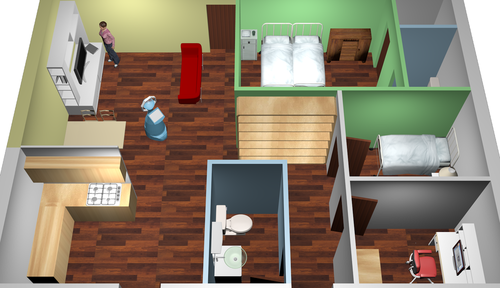
\includegraphics[width=\textwidth]{images/aruba-flat.png}
\caption{Aruba apartment visualization}
\label{aruba}
\end{figure}
As shown in Figure \cite{aruba}, the smart apartment test bed includes three bedrooms, one bathroom, a kitchen, and a living / dining room.  The apartment is equipped with motion sensors distributed approximately 1 meter apart throughout the space. The Aruba dataset was extracted from these motion sensor dataset provided by CASAS. The dataset contains the location of a person in the apartment every minute for 16 weeks.

\subsection*{Sparsification}
Aruba dataset is a large dataset as compared to an person location dataset we assume the robot will be able to generate. The Aruba dataset has recordings of every minute for 118 days, which is 161280 readings.
On the contrary the assumed dataset which will be collected by the robot by autonomously roaming in a home will be just 3-5 readings per day.
So for simulating the sparsity in the object location dataset we will sparsify the ARUBA dataset by random selecting only selecting 3-5 readings each day.

\subsection*{Visualization}
We visualize the dataset to find out if as humans we can find any patterns in the data. Since the observations are of 2 dimension(location vs time) the visualization is feasible. As explained in the section \todo{cite the central thesis}, we try to learn daily patterns by dividing the data into per hour cycle. As visualized in Figure \cite{aruba-visual} we can find that there are some prominent patterns emerging which can be learned. For example the usage of the Bedroom, Living room, outside and kitchen.

\begin{figure}[htp]
\centering
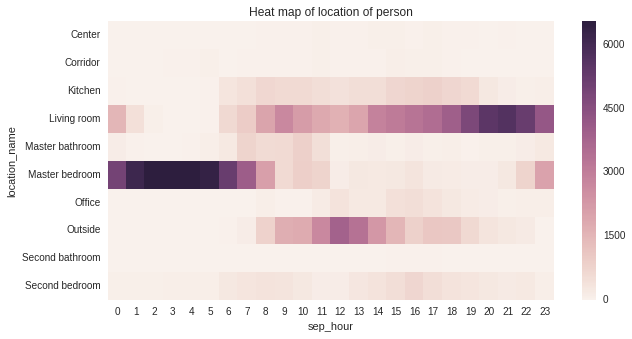
\includegraphics[width=\textwidth]{images/aruba-data.png}
\caption{Aruba Dataset Visualization : The X -axis are the locations of the home, Y-axis are the hours of the day. The intensity of the color in each box indicates the number of times the person is present in that location. Higher the intensity means more time is spent by the person in that location at that time.}
\label{aruba-visual}
\end{figure}


\section{Dirichlet Categorical model }

Dirichlet Categorical model (DCM) is a 2 level Bayesian model. The basic idea is that observations of each time period is characterized by a distribution over the possible locations.

The data are the observed human location $x_{ij}$ for $i = 1 \dots T$ time periods and then $j = 1, \dots , N$  are the observations.  We assume that the latent pattern in the persons location per period are distributed as a categorical distribution. The number of periods $T$ for our model is fixed to 24 corresponding to the number of hours in a day. 

The Dirichlet-Categorical model is the generalization of the Beta-Binomial model to multiple classes of a categorical or multinomial distribution. The conjugate prior for the categorical distribution is the Dirichlet distribution. The model estimates the posterior distribution of $\theta_i$ given our current data and prior beliefs. Our prior beliefs are encoded in the model through the hyperparameter $\alpha$, which represents pseudocounts of what we believe the data should look like – typically set as 1's for weak uniform beliefs. The graphical diagram of the model is shown in Figure \cite{dcm}

\noindent
\begin{figure}[htp]

\begin{minipage}{0.3\textwidth}
\centering

\tikz {
\node [const]                  (alpha) {$\alpha$};
\node [below=of alpha, latent]  (theta) {$\theta_i$};
\node [below=of theta, obs]     (x)     {$x_{ij}$};
\edge {alpha} {theta};
\edge {theta} {x};
\plate {trials} {(x)} {j data};
\plate {bags} {(theta)(x)(trials)} {i time};
}

\end{minipage}%
\begin{minipage}{0.7\textwidth}

\begin{equation*}
	\alpha = <1, 1, .... , 1 > 
\end{equation*}
\begin{equation*}
	\theta_i  \sim Dirichlet(\alpha)
\end{equation*}
\begin{equation*}
	x_{ij} \sim Categorical(\theta_i)
\end{equation*}
\end{minipage}
\caption{Graphical model representation of DCM. The boxes are ``plates" representing replicates. The outer plates represents hours of a day, while the inner plate represents the choice of places within each hour.}
\label{dcm}
\end{figure}



\section{Explanation : From LDA}
All the models in the thesis are based on the ``bag of words" assumption-- that the order of the data in a day can be neglected.
In language of probability theory, this is an assumption of \emph{exchangeability} for the words in the document (Aldous, 1985)

from : http://blog.nullspace.io/motivating-bayesian.html
an important class of models called exchangeable models are guaranteed by de Finetti’s theorem to decompose cleanly into the definition of the Bayesian framework.

One reason exchangeability is interesting is because prima facie, although it seems to be similar to the assumption of iid, it is actually much richer, and much less restrictive. Consider, for example, if we have a document whose words have been shuffled. Intuitively, if we see an Arabic word, then even it is much more likely that we will encounter other Arabic words elsewhere in the document, since there is a reasonable probability the document itself is in Arabic. The assumption of iid does not capture this, because the words are assumed to be completely independent. Exchangeability doesn’t assume independence, however, only that ordering doesn’t matter, so this will be captured in a model that is exchangeable.

This is a critical aspect of Bayesian inference that many people simply don’t understand, and it has all sorts of consequences, like making Bayesian nonparametrics possible, and making conditional probabilities uncomputable in general. It is so convenient to think of this class of problems as Bayesian that it seems like a crime to not use Bayesian inference.


\begin{itemize}
	\item Generative probabilistic model
	\item three-level hierarchical Bayesian model
	\item 
\end{itemize}


\section{Discussions}

http://andrewgelman.com/2016/08/22/bayesian-inference-completely-solves-the-multiple-comparisons-problem/
http://andrewgelman.com/2013/11/21/hidden-dangers-noninformative-priors/

The point of the story in that slide is that flat priors consistently give bad inferences. Or, to put it another way, the routine use of flat priors results in poor frequency properties in realistic settings where studies are noisy and effect sizes are small.
\label{sec:}

% section  (end)
\end{document}

